
% This is the main file to setup the document.
% Document organization and appearance settings are all done here
% Each chapter is a separate tex file, all linked together here


% Preamble (document settings) -----------------------------------------------------------
% Document type and font --
\documentclass[12pt,a4paper,twoside]{report}

\usepackage[margin=1in]{geometry}

\pagestyle{plain}

\font\Bold=cmbx10 scaled \magstep3
\def\EndOfProof{\nolinebreak\ \hfill\rule{1.5mm}{2.7mm}}
\def\endOfProof{\ \hfill\rule{1.5mm}{2.7mm}}
\def\proof{\noindent \textbf{Proof:}\quad}

\usepackage{subfigure,amssymb,amsmath,epsfig,fancyhdr}
\usepackage[utf8]{inputenc} %utf-8 encoding for ASCII symbols
\usepackage{svg}
% insert packages here --
\usepackage{graphicx}       %for handling images

\usepackage{breakcites}     %to avoid citations extending into the margin

\usepackage{sidecap}        %to enable side captions on figures

\usepackage{setspace}       %to enable doublespacing   

\usepackage[
backend=biber,
mincitenames=1,maxcitenames=1,
style=ieee,
citestyle=numeric
]{biblatex}       %use the biblatex package

\addbibresource{references.bib}   %path to the bib file



\usepackage{hyperref}       % to create a linked table of contents
\hypersetup{
    colorlinks,
    citecolor=black,
    filecolor=black,
    linkcolor=black,
    urlcolor=black
}

% Set path to images
\graphicspath{ {images/} }  % Direct to the main image folder, always good to create sub-folders to organize images for individual chapters


% End of preamble
%-------------------------------------------------------------------------------------------
\usepackage{pgfplots}
\usepackage{csvsimple}
\usepackage{multirow}


\begin{document}

% Making title page


\begin{titlepage}
\begin{center}
\begin{doublespacing}

       \begin{figure}
       \centering
       \includegraphics[width=0.7\textwidth]{images/Nanyang_Technological_University.png}
       \end{figure}
       
       
       \vspace*{5mm}
       \LARGE{\textbf{Transfer Learning for Non-Autoregressive Sequence Generation\\}}
       {\large{\\Qualifying Examination Report\\
        Submitted to the School of Computer Science and Engineering\\
        of the Nanyang Technological University
        }}

       \vspace{15mm}
       \large{by}\\
       
       \vspace{15mm}
       {\Large\textbf{Andrew Koh Jin Jie}}

       \vspace{20mm}

       {\large{for the Confirmation for Admission \\
        to the Degree of Doctor of Philosophy}\\}

       \vfill
       \large{Month, 2021}
       
\end{doublespacing}
\end{center}
\end{titlepage}


% Starting frontmatter:
% Abstract goes here
\doublespacing

\thispagestyle{plain}
\begin{center}
    \vspace{0.9cm}
        \textbf{\Large{Abstract}}
\end{center}

Autoregressive methods have been the defacto decoding method for sequence generation. However, with the increasingly bigger models in the recent years, the need for non-autoregressive models has become even more pressing in order to save time and computational power. In this work, we examine transfer learning as a method to convert an autoregressive model to a non-autoregressive model. We also propose a novel decoding method for our architecture. Finally, we study the effect of freezing certain layers in the autoregressive models during transfer learning.
\addcontentsline{toc}{section}{\textbf{Abstract}}
\pagenumbering{roman}   % Roman page numbering to start from abstract onwards

\singlespacing          % keep pre-content single spaced
\listoffigures          % generate list of figures
\addcontentsline{toc}{section}{\textbf{List of Figures}}

\listoftables           % generate list of tables

\printbibliography[keyword=myref,title={My Publications}]


\addcontentsline{toc}{section}{\textbf{List of Tables}}

% End of frontmatter

% Insert table of contents
\tableofcontents

% Main matter starts here --
% Inserting individual chapters. Mention chapter titles here and simple link the chapter's tex file
\doublespacing
\chapter{Introduction}     % Mention chapter title here
\pagenumbering{arabic}    % We want Arabic numerals for main matter page numbering

This section serves as a brief preamble of the motivation behind this research topic, and delineates the structure of this report. 

\section{Motivation} \label{sec:motivation}
Non-autoregressive sequence generation is an emerging research area in its infancy. It refers to the speeding up the decoding of the sequence generation by generating parts of, or the whole of the sequence in one decoding step. Thus far, it is typically used in conjunction with variants of the transformer model, and mainly applied in the domain of machine translation. However, it is noted \cite{wang_semi-autoregressive_2018} that while the non-autoregressive literature often falls into the domain of machine translation, the non-autoregressive decoding process is not limited to machine translation, and can in fact be applied to other tasks such as summarization, question answering, or any task which involves generating a sequence.

Research in non-autoregressive sequence generation is crucial as it tackles one major drawback of current autoregressive sequence generation methods. Specifically, this drawback refers to the huge bottleneck during decoding; sequences in autogressive sequence decoding are generated token by token, with each token requiring one forward pass through the model. This inhibits parallelism during inference, and the computation cost is compounded with different decoding methods and the size of the model. Tackling this bottleneck would result in many benefits, such as a greatly increased decoding speed, savings in time, money, and computational cost, and a lower barrier to entry for using sequence generation.

However, non-autoregressive sequence generation unfortunately suffers from multiple problems. Removing the autoregressive factorization across time or decoding steps causes the model to depend only on the source sentence for decoding, and this greatly reduces the quality of the generation. These problems, along with their solutions, will be discussed in subsequent sections.

\section{Report Outline} \label{sec:report_outline}
This report will explore and discuss these topics. In Chapter 2, we will briefly introduce the background of autoregressive methods and models, and popular training methods such as transfer learning. We will examine the limitations of these methods and models and introduce the need for non-autoregressive methods. We will then provide a comprehensive literature review of non-autoregressive models along with their proposed solutions. In Chapter 3, we will discuss our motivation and thought process behind our proposed approach. In Chapter 4, we will go through our methodology, implementation details, and experimental results. Finally, in Chapter 5, we conclude and propose several avenues of research for future work.

% While there has been non-autoregressive methods such as CTC applied to automatic speech recognition, there is  


% Insert images like this:
% \begin{figure}[h!]
%     \centering
%     \includegraphics[width=0.50\textwidth]{images/chap01_images/PaleBlueDot.png}
%     \caption{Photograph of planet Earth taken on February 14, 1990, by the Voyager 1 space probe from a record distance of about 6 billion kilometers.}
%     \label{fig: PaleBlueDot}    
% \end{figure

% This is some random reference (\cite{sanchez2011introduction}). \textcite{parish2009propagation} is an example of how to use textcite. % Link to the chapter tex file

\chapter{Literature review} 

% Literature Review 

% Talk about standard RNNs, pre-transformers era? Why was there no NAT in this era? 

% Brief intro about transformers? Why is it so ubiquitous in today’s research 

% Problems in NAT 

% Removal of Autoregressive factorization across time 

% Multimodality problem 

% Where has NA-solution been done before? 

% Solutions 

% Iterative Refinement 

% Semi-autoregressive - Trade off between faster generation and quality 

% Distilled training data – reduce number of modes 

% Limitations of this solutions – iterative refinement requires complex solutions and architectures. 

This chapter aims to provide a comprehensive literature review of research done for non-autoregressive transformer models. This section will first briefly cover methods for sequence to sequence prior to the era of the transformer \cite{vaswani_attention_2017}; for which the need for non-autoregressive methods was not so pressing. After which, we will provide a summary of the transformer architecture \cite{vaswani_attention_2017} and then examine different non-autoregressive methods.

It is important to note that non-autoregressive methods are not completely new and unheard of. There has been methods and algorithms proposed in other domains. We will dedicate the last section of this chapter to those methods. 



\section{Background and History} \label{sec:background}
\subsection{Autoregressive Methods for sequence to sequence generation} \label{subsec:background1}
Prior to the advent of transformers models in 2017 \cite{vaswani_attention_2017}, the defacto models to use for sequence to sequence generation were variants of Recurrent Neural Network \cite{elman_distributed_1991}, such as the Long Short Term Memory \cite{lstm_original}, Gated Recurrent Unit \cite{gru_paper}. At inference time, these models generate words via an autoregressive factorization, following the equation:

\begin{equation} \label{eqn:autoregressive_factorization} P(y|x) = \prod_{t=1}^{T}p(y_t|y_{<T},x) \end{equation}

This autoregressive factorization assumes casual conditional dependence between the current decoding step and the output of the previous decoding step, thus generating the sequence from left to right. This implementation also permits the training of the models to be relatively straightforward by simply minimizing the negative log likelihood of Equation \ref{eqn:autoregressive_factorization}, allowing for training methods as teacher forcing \cite{williams_learning_1989_teacher_forcing}.

The need for non-autoregressive methods were not as vital then, as the autoregressive factorization were thought to be one of the advantages of RNNs variants in order to induce temporal invariance \cite{battaglia_relational_inductive_biases_2018} in the model. The size of RNN models were also relatively smaller compared to today. The need for non-autoregressive methods stemmed from the increased popularity in model variants of the transformer \cite{vaswani_attention_2017}. In the next subsection, we will concisely cover the transformer architecture, and explain the demand for non-autoregressive methods.


\subsection{Transformer}\label{subsec:background2}
\textcite{vaswani_attention_2017} proposed the transformer in 2017. Since then, many model variants have been introduced to take advantage of its exceptional language modeling capabilities, At the core of the transformer architecture is an unique self-attention mechanism used to model dependencies independent of their respective positions in the input or output sequence \cite{vaswani_attention_2017}.The transformer follows an encoder-decoder structure \cite{cho_learning_2014_encdec, sutskever_sequence_2014_encdec, bahdanau_neural_2016_encdec} consisting of stacks of self-attention, feed-forward, and layer normalization.This formulation allows the transformer to scale up to huge sizes on huge training data by leveraging on hardware and the ability to be parallelized during the training process. 
% should i go into more specific detail about transformer?


Since then, many different transformer variants \cite{wolf-etal-2020-transformers} have been proposed for a multitude of purposes. For instance, BERT \cite{devlin_bert_2019} gave rise to the trend of using contextualized word embeddings, which soon proved to be superior to static word embeddings such as word2vec \cite{mikolov_efficient_2013_word2vec}. As a consequence, transfer learning became a popular method to adapt the publicly available pretrained BERT model for fine-tuning on downstream tasks such as word sense disambiguation \cite{yap_adapting_2020}. Transformers have also been applied to sequence to sequence tasks. Notable models include GPT-2 \cite{radford_language_nodate_gpt2}, GPT-3 \cite{brown_language_2020_gpt3}, both of which was trained on a huge corpus of text data and has since surpassed many benchmarks and shown potential for few-shot learning for many tasks such as story generation and even simple arithmetic.

\subsubsection{An example of Transfer Learning}\label{subsubsec:transfer_learning_me}

\label{subsec:transfer_learning}
\begin{figure}[hpbt!]
    \centering
    \includegraphics[scale=0.5]{images/chap02_images/transfer_learning_toy_example.png}
    \caption{An straightforward example of how transfer learning is usually done. A language model is pretrained first using a language modeling task. These pretrained language models are availably readily online. Thereafter, the pretrained language model is finetuned on a downstream task. In this example, it is trained on sentiment analysis and is used to output a sentiment score.}
    \label{fig:transfer_learning_toy_example}
\end{figure}
Transfer learning \cite{zhuang_comprehensive_2020_transfer_learning} is a common machine learning technique which aims to adapt the information in a trained model to a related domain. In today's Natural Language Processing landscape, transfer learning is made ubiquitous and popular by the ease of access of pretrained language models like BERT \cite{devlin_bert_2019}. Using transfer learning (Toy example in Figure \ref{fig:transfer_learning_toy_example}) allows us to use pretrained models and possibly save lots of compute time.

\textcite{yap_adapting_2020} used transfer learning to adapt a BERT \cite{devlin_bert_2019} pretrained model to a word sense disambiguation task. Pretraining is done by training BERT trained on gigabytes of text data on a masked language modeling task, allowing it to learn contextualized word representations. The pretrained BERT is publicly available at many open source repositories. \textcite{yap_adapting_2020} then fine-tuned the pretrained BERT model on the gloss selection task. In doing so, the gloss selection task allowed the BERT model to break state of the art on the word sense disambiguation task. 

Transfer learning is a tried and tested method to adapt models across different domains. In this work, we will also utilize transfer learning. Section \ref{subsec:transfer_learning} covers this usage in details.

\subsection{Drawbacks of the transformer} \label{subsec:drawbacks_transformer}

\subsubsection{Loss of inductive bias} \label{subsubsec:drawback1_inductive_bias}
Unlike the recurrent neural network whose recurrent structure induces temporal invariance and locality bias in the model \cite{battaglia_relational_inductive_biases_2018}, the feed-forward layers and self-attention layer in the transformer does not has any relational inductive bias \cite{battaglia_relational_inductive_biases_2018}. In other words, the transformer sacrifices the temporal invariance for greater modeling capacity and scaling potential. 

\subsubsection{Steady increase of model size over the years} \label{subsubsec:drawback2_increasing model size}

%todo plot model sizes?
The ease of scaling of transformers to hundreds of gigabytes in data has also led models sizes to steadily increase. The original transformer \cite{vaswani_attention_2017} had only 66 million parameters. BERT, in 2018, \cite{devlin_bert_2019} had 110 million parameters. By 2020, Turing-NLG had 17 billion\footnote{https://www.microsoft.com/en-us/research/blog/turing-nlg-a-17-billion-parameter-language-model-by-microsoft/} \cite{ganesh2020compressing_turingNLG_param_ref}, and GPT-3 \cite{brown_language_2020_gpt3} had an even larger 175 billion, dwarfing its predecessors significantly in size. Recently in 2021, Microsoft released the Switch Transformer \cite{fedus2021switch}, which has a gigantic trillion parameters.

This trend has raised questions in the research community about the practicality and impact \cite{schwartz_green_ai_2019} of large models. These large models are expensive to run and a large amount of computational power and memory is required just for a single forward pass through the model. As a result, there has been work looking to compress these large models, either via knowledge distillation \cite{hinton_distilling_2015} to train a smaller model \cite{sanh_distilbert_2020}, or by pruning \cite{rogers_primer_in_bert_2020,chen_lottery_2020,frankle_lottery_2019} models to reduce computation.

In a similar vein, non-autoregressive transformer models aim to speed up generation by generating more or all tokens in a single forward pass of the model. This allows for huge savings in computational power compared to  autoregressive transformer sequence to sequence models \cite{vaswani_attention_2017, brown_language_2020_gpt3, radford_language_nodate_gpt2} which can only generative one token per forward pass.



\section{Non-autoregressive Transformer sequence to sequence Models} \label{sec:NAT model}

\subsection{Problem Definition} \label{subsec:problem_def}
Non-autoregressive sequence generation aims to speed up decoding by removing the autoregressive factorization in Equation \ref{eqn:autoregressive_factorization}. At its most simplest and naive form, non-autoregressive generation can be formulated as:

\begin{equation}
\label{eqn:naive_non_autoregressive_formulation} 
P(Y|X) = \cdot \prod_{t=1}^{T}p(y_t|x_{1:T^\prime})
\end{equation}

where generation is only dependent on the very first input sequence. This formulation is straightforward, and training can be done similarly to autoregressive training by minimizing the negative log-likelihood.

However, the removal of conditional dependence across time has created several problems at the cost of faster generation. In the next subsection, we will explain these problems.

\subsection{Obstacles to realizing a deployable non-autoregressive sequence to sequence model} 
\label{subsec:obstacles_NAT}
In this section, we will examine different problems arising from the lack of the autoregressive factorization in non-autoregressive sequence generation.
\subsubsection{Length Prediction} \label{subsubsec:nat_prob_length}
As mentioned in Section \ref{sec:background}, autoregressive sequence generation decodes the sequence token by token. The decoding algorithm stops when the end of sequence token is generated in the latest decoding step. This heuristic is uncomplicated and works well practically. On the other hand, non-autoregressive sequence generation is not afforded this advantage as either any part or the whole of the sequence is generated in one decoding step. Therefore, there is a need to predict or assume the length of the output sequence in non-autoregressive sequence generation. 

\textcite{gu_non-autoregressive_2018} circumvents this by naively modelling the output sequence length using a separate conditional distribution $P_L$. Thus, Equation \ref{eqn:naive_non_autoregressive_formulation} becomes:
\begin{equation}
\label{eqn:gu_non_autoregressive_formulation} 
P(Y|X;\theta) = p_L(T|x_{1:T^\prime};\theta) \cdot \prod_{t=1}^{T}p(y_t|x_{1:T^\prime};\theta)
\end{equation}

Several authors choose to espouse this approach of modeling the length of the output sequence, either by dynamically changing the output sequence length with each decoding step using a length heuristic or prediction module \cite{gu_levenshtein_2019,chan_kermit_2019,chan_multilingual_kermit,ran_learning_to_recover_2020,stern_insertion_2019,zhou_improving_2020_with_monolingual_data, ran_guiding_2020_reordering,ma_flowseq_2019}, or by predicting a static output sequence length \cite{gu_non-autoregressive_2018,zhou_improving_2020_with_monolingual_data,ghazvininejad_mask-predict_2019, qian_glancing_2020}. Other methods assume a fixed sequence length during decoding \cite{wang_semi-autoregressive_2018,guo_non-autoregressive_2020_image_captioning,saharia_non-autoregressive_2020_latent_alignment,chan_imputer_2020,bao_non-autoregressive_2019_position_learning, guo_fine-tuning_2019_curriculum,ding_context-aware_2020} at the cost of flexibility of the generated sequence and a potential issue of choosing the wrong sequence length.

\subsubsection{Multi-modality Problem} \label{subsubsec:nat_prob_multimodal}
An arguably bigger problem to non-autoregressive sequence generation is its strong decline in generation quality. Autoregressive sequence generation implicitly models the strong casual correlation across time \cite{gu_non-autoregressive_2018} when decoding. Removing the autoregressive factorization causes the model to lose that ability. As a result, the multi-modality problem arises \cite{gu_non-autoregressive_2018, zhou_understanding_2020}. This problem often manifests itself in sequence generation as token repetition \cite{ran_learning_to_recover_2020}.

\begin{figure}[hpbt!]

    \centering
    \includegraphics[width=\textwidth]{images/chap02_images/AT_vs_NAT.png}
    \caption{Comparison of the decoding process in an autoregressive model (left) and a non-autoregressive model (right). The non-autoregressive model is able to generate the next token based on the sequence generated in the previous step, while the non-autoregressive model does not do so and hence assumes conditional independence between each output token.}
    \label{fig:AT_vs_NAT}
\end{figure}

\begin{figure}[hpbt!]

    \centering
    \includegraphics[width=\textwidth]{images/chap02_images/AT_vs_NAT_distributions.png}
    \caption{A simplified view of how the multimodality problem manifests in non-autoregressive sequence generation. 'Danke', 'Vielen', 'schön' are the multiple modes of the  initial probability distribution. \textbf{Left:} Autoregressive sequence generation decodes a single mode from the multiple available modes. In subsequent decoding steps, the number of modes in the distribution is reduced. \textbf{Right:} Non-autoregressive sequence generation typically has to choose multiple tokens from multiple modes, and therefore leads to repetitive tokens in its generation.}
    \label{fig:AT_vs_NAT_distribution}
\end{figure}
% not working
% \begin{figure}[htbp]
%   \centering
%   \includesvg{images/chap02_images/AT_vs_NAT.svg}
%   \caption{svg image}
% \end{figure}


The multi-modality problem is defined by \textcite{gu_non-autoregressive_2018} as the inability to accurately reflect the conditional independence of each word in the sequence using a single target distribution. For example \cite{gu_non-autoregressive_2018}, the English phrase 'Thank you' can be translated correctly into `Danke', `Danke schön', or `Vielen Dank' in German. As an non-autoregressive model would most likely generate the whole sequence in one decoding step, it is possible that `Danke Dank' or `Vielen schön' gets produced. This is because there is no conditional dependence between the first word and the second word. In other words, the generation of the second word does not rely on the first word. This is depicted in Figure \ref{fig:AT_vs_NAT}. 

`Danke', `Vielen', `schön' are all highly possible outputs of the model, and hence are referred to as `modes'. At decoding time, the non-autoregressive model is not prohibited from choosing conflicting modes to use in the output sequence, nor is it able to determine if a mode has already been or will be chosen for another position. Figure \ref{fig:AT_vs_NAT_distribution} further illustrates this phenomenon. Therefore, the problem of decoding conflicting modes is referred to as the multi-modality problem.

\section{Solutions and Approaches} \label{sec:solutions}

In this section, we will discuss the different approaches towards the problems metioned in Section \ref{subsec:obstacles_NAT}. Many of these approaches are used in conjuction with the other approaches mentioned below.
% Iterative Refinement 
% Semi-autoregressive - Trade off between faster generation and quality 
% Distilled training data – reduce number of modes 
% Fertilities  
% Limitations of these solutions – iterative refinement requires complex solutions and architectures. 

\subsection{Sequence Level Knowledge Distillation}
\label{subsec:sol1_slkd}
%put  image on example of how slkd is done here
\begin{figure}[h!]
    \centering
    \includegraphics[width=\textwidth]{images/chap02_images/seq_level_kd.png}
    \caption{Sequence level knowledge distillation. The original training data is fed through an autoregressive teacher model first. The distilled corpus is formed by collecting all the generated outputs paired with the same original source sequence.}
    \label{fig:slkd}
\end{figure}


Knowledge Distillation is the most common approach used to tackle the multi-modality problem mentioned in Section \ref{subsubsec:nat_prob_multimodal}. With the exception of \cite{ran_learning_to_recover_2020}, almost all work in non-autoregressive research \cite{ren_study_2020_comma, gu_non-autoregressive_2018, gu_levenshtein_2019, guo_non-autoregressive_2020_image_captioning, bao_non-autoregressive_2019_position_learning, wang_semi-autoregressive_2018,saharia_non-autoregressive_2020_latent_alignment, chan_kermit_2019, chan_multilingual_kermit, ghazvininejad_mask-predict_2019,stern_insertion_2019, zhou_improving_2020_with_monolingual_data, ran_guiding_2020_reordering, ma_flowseq_2019, qian_glancing_2020, guo_fine-tuning_2019_curriculum, ding_context-aware_2020} use sequence level knowledge distillation \cite{kim_sequence-level_2016_knowledge_distillation} for training in the domain of machine translation. Sequence level knowledge distillation is done by first training a teacher autoregressive model, and then passing the source training data through the autoregressive model to get the predicted sequence from the model. These generated outputs are paired with the same source sequences and used as distilled training data for the non-autoregressive model. This process is shown in Figure \ref{fig:slkd}.

\textcite{zhou_understanding_2020} quantified the effectiveness of sequence level knowledge distillation in his work. They found empirical evidence that the use of the autoregressive model to generate a new set of training data significantly reduced the number of modes in the new training data. Specifically, \textcite{zhou_understanding_2020} used a measure of complexity and faithfulness to the original training data. They found that models with low capacity such as the vanilla non-autoregressive model \cite{gu_non-autoregressive_2018} prefered training data with lower complexity, while models with higher capacity such as the Levenstein Transformer \cite{gu_levenshtein_2019} preferred training data with higher complexity. Using distilled data greatly mitigates the multi-modality problem mentioned in Section \ref{subsubsec:nat_prob_multimodal}, thereby boosting the quality of the generated sentence.

\subsection{Fertilities} \label{subsec:sol2_fertilities}
\textcite{gu_non-autoregressive_2018} first introduced the vanilla non-autoregressive transformer which aims to tackle the multimodality problem using fertilities. Fertilities determine the number of words in the target sentence that each word in the source sentence corresponds to. Therefore, the length of the target sequence can be easily calculated by summing the fertilities, while at the same time providing the model with an intermediate factorization of the output space. \textcite{gu_non-autoregressive_2018} modeled the fertilities $p_F(f_{t^\prime}|x_{1:T^\prime})$ using a simple feedforward linear layer with a softmax classifier at output encoder embedding of each input token. The casual mask of the decoder was also removed so that the whole sequence could be generated simultaneously. 

However, this approach was criticized as limited in terms of expressiveness \cite{ma_flowseq_2019} and was unable to properly model the interdependence between words in the output sequence. Subsequent work mostly focused on other approaches and used variants of iterative refinement algorithms. 

\subsection{Iterative Generation} \label{subsec:sol3_iterative_generation}
Due to the limited modeling capacity of fertilities, not many research work espoused this approach. Instead, many authors chose to deal with a tradeoff between the number of decoding steps and generation quality via the iterative refinement approach. Typically, the more the number of decoding steps, the higher the quality of the sequence. There are several methods along this approach. Most work chose to increase the number of decoding steps in order to improve the generation quality. It is hypothesized \cite{ghazvininejad_mask-predict_2019} that iterative sequence generation helps to collapse the modes in the distribution, thus alleviating the multi-modality problem. There are two main approaches, left-to-right non-autoregressive sequence generation, and arbitary-position non-autoregressive sequence generation. This is depicted in Figure \ref{fig:leftright_vs_arbitrary}.


\begin{figure}[hbtp!]
    \centering
    \includegraphics[width=\textwidth]{images/chap02_images/leftright_vs_arbitrary.png}
    \caption{Visualization of a simplified decoding process of the two non-autoregressive sequence generation approaches. \textbf{Top:} Left to right non-autoregressive sequence generation. It resembles the left-to-right autoregressive sequence generaiton, except that more than one token is predicted with decoding step. \textbf{Bottom:} Arbitrary-Position NAR sequence generation. A blank canvass is fed to the decoder and the decoder fills in the canvass at any possible. Note that this is simplified, most models use a more complicated heuristic.}
    \label{fig:leftright_vs_arbitrary}
\end{figure}
%put image of left-right vs arbitary position here


\subsubsection{Left-to-right non-autoregressive Sequence Generation} \label{subsubsec:sol3_iterative_generation_left2right}
This method resembles left-to-right autoregressive sequence generation, except that groups of tokens are generated with every decoding step. This approach is not common.

Currently, only the Semi-Autoregressive Transformer \cite{wang_semi-autoregressive_2018} espouses this approach. The Semi-Autoregressive Transformer uses a relaxed causal attention mask along with a group level chain rule to predict the next group of tokens. Using different forms of attention masks, the Semi-Autoregressive Transformer performs long and short distance prediction of tokens. In this work, we also use left-to-right non-autoregressive sequence generation.

\subsubsection{Arbitary-position non-autoregressive sequence generation} \label{subsubsec:sol3_iterative_generation_arbirtary_position}
Models in this section generate tokens on a canvas. The generated tokens can be placed anywhere in the sequence; it does not have to be from left to right. The positions of the generated tokens are decided either via a heuristic or a classification task depending on the setup of the model. 

These are some examples of models espousing this approach. The Levenshtein Transformer \cite{gu_levenshtein_2019} takes inspiration from the Levenshtein distance \cite{Levenshtein1965BinaryCC_lev_distance} and iteratively suggests token insertion and deletion operations on a canvas. KERMIT \cite{chan_kermit_2019, chan_multilingual_kermit} and the Insertion Transformer \cite{stern_insertion_2019} also takes a similar insertion-only approach by placing predicted tokens in between slots in a sequence.  Similarly, the Imputer \cite{chan_imputer_2020},a latent alignment model, assumes a monotonic mapping between token alignment predictions and the target sequence in order to fill in a canvas. These models work relatively well, however, they are complex to train and use.

% lev trans, semi-auto, latent alignment, imputer, kermit, multi-kermit, insertion, 

\subsection{Supplementing generation with external knowledge} \label{subsec:sol4_external_knowledge}
% position learning, reorder, monolingual, flowseq,
The methods in this section incorporates external knowledge via latent variables into the encoder or decoder of the transformer to improve non-autoregressive sequence generation. Unless mentioned otherwise, all models in this section follow that of the vanilla non-autoregressive transformer \cite{gu_non-autoregressive_2018}; the whole sequence is generated in one decoding step. 

PNAT \cite{bao_non-autoregressive_2019_position_learning} creates a position predictor module for the model to model the positions of the sequences. The module produces a latent variable which is then incorporated into the decoder input.

In another vein, \textcite{zhou_improving_2020_with_monolingual_data} supplements the non-autoregressive transformer by adding more data from a monolingual dataset of the source language. The additional dataset is fed through a separate trained autoregressive model to produce the sequences in the target language. The additional data is then used in conjuction with the original parallel dataset to train the model.

Unlike all the other approaches, Flowseq \cite{ma_flowseq_2019} further reinvents the wheel by using flow based generative models \cite{rezende_variational_2016_flow} instead of the transformer. Using a chain of invertible operations, a simple distribution is modelled into a complex distribution \cite{ma_flowseq_2019}. The use of generative flow also allows the use of Recurrent Neural Networks, while still keeping the non-autoregressive property. 


\subsection{Post-Editing} \label{subsec:sol5_post_editing}
Post-editing, also commonly known as sequence refinement, is a relatively recent technique applied to non-autoregressive generation. It refers to modifying or improving the sequence that has been already generated. This can be done in the next decoding step as part of the generation process.

As mentioned in Section \ref{subsubsec:sol3_iterative_generation_arbirtary_position}, \textcite{gu_levenshtein_2019} applies post editing as part of its Levenshtein Transformer. It uses a token deletion operation to dynamically delete tokens that are deemed to be incorrect, and the token insertion operation can add to the sequence. 
Mask-Predict \cite{ghazvininejad_mask-predict_2019} generates the whole sequence in one decoding step, but indicates uncertainty in its generation by masking some tokens out. In the next decoding step, the model re-predicts the masked tokens. RecoverSAT \cite{ran_learning_to_recover_2020} also generates segments of tokens simulateously, then removing repetitive segments indicated by a deletion token. Lastly, the Glancing Transformer \cite{qian_glancing_2020} adopts a 3 stage decoding process. First, the model decodes the whole sequence. Then, it conducts a novel glancing operation to determine which words are likely to be wrong. Finally, the models samples from the probability distribution to update the sequence.
% lev trans, mask predict, learning to recover,


\chapter{Exploring the use of Transfer Learning for Non-Autoregressive Machine Translation}
% Simple adaptor layer for ngram prediction 

% Motivation – words often cluster together as a phrase- ngram 

% Predicting a future and past window vs future ngram prediction (prophet-net) 

% Past window allows us to perform post editing 

% Transfer learning 

% If original data has lots of modes, will it be faster to reduce the number of modes very transfer learning? 

% Using graph information 

% Syntax information might help circumvent the lack of autoregressive factorization 

In this chapter we discuss our methodology, inspiration and thought process behind our proposed approach.
\section{Motivation}
The research work mentioned in Section \ref{sec:NAT model} often reinvents the wheel and proposes novel model architectures. These new architectures are typically trained from scratch on the same data as their autoregressive counterparts, and the number of parameters of the novel models are often increased significantly. The complexity of the models are also not straightforward and simple to understand. This precludes the use of many autoregressive models that have already been trained. 

Given that it has been asserted by research \cite{gu_non-autoregressive_2018,zhou_understanding_2020} that the output distribution of an autoregressive model is multi-modal, the next natural step is to wonder if we can reduce the multi-modality in an already trained autoregressive model for it to work in a non-autoregressive setting. To this end, we investigate the use of transfer learning.



\section{Transfer Learning} \label{subsec:transfer_learning}
As mentioned in Section \ref{subsubsec:transfer_learning_me}, transfer learning \cite{zhuang_comprehensive_2020_transfer_learning} is a common machine learning technique which aims to adapt the information in a trained model to a related domain. In today's Natural Language Processing landscape, transfer learning is made ubiquitous and popular by the ease of access of pretrained language models like BERT \cite{devlin_bert_2019}. Using transfer learning (Toy example in Figure \ref{fig:transfer_learning_toy_example}) allows us to use pretrained models and possibly save lots of compute time.

\subsection{Adaptor Layers}\label{subsec:adaptor_layers}
There has been work looking into how transfer learning can be made more efficient. Adaptor layers \cite{bapna_simple_2019_adaptor1,houlsby_parameter-efficient_2019_adaptor2} were one of the proposed ideas . Simply put, adaptor layers are a small module of parameters which can be plugged into each layer of the transformer architecture. This allowed most of the pretrained transformer to be frozen, and allowing us to train only the adaptor module. Freezing most of the model leads to significant reduction in training time and computational power. In Section \ref{subsec:architecture}, we will explain how the adaptor modules are incorporated into the model. 

\section{N-gram language modeling} \label{sec:ngram_lm}
N-grams refer to contiguous groups of words or  phonemes that happen together in a sentence. Traditionally, n-grams have been used for static word emebddings such as word2vec \cite{mikolov_efficient_2013_word2vec} and fastText \cite{bojanowski_enriching_2017_fasttext}. Both algorithms make use of co-occurrence information such as n-grams in order to compute vector representation of a word. In the domain of language sequence evaluation, many evaluation methods such as BLEU \cite{papineni_bleu_2002} make use of n-grams to score a pair of reference text and generated text.

More recently, ProphetNet \cite{qi_prophetnet_2020} proposed a novel future n-gram prediction task for the model to predict future n-grams. We adopt a variation of this task for non-autoregressive sequence generation and will explain it in Section \ref{sec:past_future_n-gram_lm}.


\section{Research Questions}
Given the availability of pretrained language models, it would be extremely convenient and efficient if we could adapt these pretrained autoregressive language models in non-autoregressive research. Therefore, we pose these research questions:

\begin{enumerate}
    \item Is it possible to convert a pretrained autoregressive model to a non-autoregressive model using transfer learning?
    \item Is the n-gram prediction task sufficient for non-autoregressive sequence generation?
    \item Which layers in the transformer architecture are instrumental for better performance in non-autoregressive sequence generation?
\end{enumerate}

We explain our methodology to answer these questions in the next chapter.

\chapter{Methodology}


% \begin{filecontents*}{main_NAT_experiments.csv}
% Window Size,"1,1","2,2","4,4","8,8","0,1","0,2","0,4","0,8"
% distilled data from scratch,27.04,25.48,22.52,18.13,26.94,25.76,23.55,19.63
% distilled data from pretrained,27.44,25.75,22.72,16.7,26.37,26.45,23.87,19.5
% original data from scratch,26.14,22.58,16.92,7.18,26.12,23.26,18.72,9.45
% original data from pretrained,26.27,23.1,17.15,6.85,23.57,23.41,18.18,9.45
% \end{filecontents*}


Inspired by the abovementioned in Section \ref{subsec:transfer_learning}, we present our suggested approach and model architecture. 


\section{Past and Future N-gram Language Modeling Task} \label{sec:past_future_n-gram_lm}

\begin{figure}[hpbt!]

    \centering
    \includegraphics[width=\textwidth]{images/chap04_images/ngram language modeling.png}
    \caption{An example of the Past and Future N-gram Language modeling task. The model predicts a past window and a future window given the input.}
    \label{fig:n-gram_lm}
\end{figure}

We introduce a variant of the N-gram prediction task \cite{qi_prophetnet_2020}. In the Past and Future Language Modeling task, the model is trained to predicted a window size of tokens. An example is shown in \ref{fig:n-gram_lm}. The configuration of the window is specified by the user. For simplicity, we set the window sizes to be powers of 2. Half of the window is used to predict past tokens, and the other half is used to predict the future tokens. 

There are several reasons behind this design. Firstly, predicting past tokens allows us to do sequence refinement (as mentioned in Section \ref{subsec:sol5_post_editing}), while speeding up generation. A window size of 1/1 (Future window of 1 and back window of 1) defaults to autoregressive generation while allowing the capability for post editing. A window size of 4/4 (Future window of 4 and back window of 4) speeds up generation by 4x relative to autoregressive generation. We also experiment with non-uniform window sizes; such as 4/2 (future window size of 2 and past window size of 4). Secondly, this enable us to utilize the autoregressive decoding framework without having to reinvent the wheel and significantly introduce changes in the model. Decoding of a sequence can halt when there is an end of sequence token generated in the future window. Lastly, this objective is straightforward, and allows for transfer learning from autoregressive models.

\section{Model Architecture}\label{sec:architecture}

\begin{figure}[hpbt!]

    \centering
    \includegraphics[width=\textwidth]{images/chap04_images/adaptor_module.png}
    \caption{Model Architecture. The transformer encoder and decoder is kept the same. We append the adaptor module to the output of the transformer decoder. In this example, the window size of model is 2/2 (past window of 2 and future window of 2).}
    \label{fig:AT_vs_NAT}
\end{figure}

We keep the transformer architecture the same. However, instead of applying a softmax over the last hidden state in the decoder, we pass all hidden states to the adaptor module. The adaptor module is adapted from \textcite{houlsby_parameter-efficient_2019_adaptor2}. The hidden states are down-projected to a hidden size of a specified hyperparameter, passed through the non-linearity GeLu, and then up-projected back to the original hidden size. A residual connection is used to add the original hidden states to the up-projection. This architecture is simple and allows for transfer learning to be done using publicly available models.

\section{Decoding Methods} \label{sec:decoding_methods}
Typically, beam search is used for decoding in autoregressive models. Other non-autoregressive methods like the Levenshtein Transformer \cite{gu_levenshtein_2019} are unable to use beam search as beam search requires a contiguous beam of tokens to be scored at each decoding step. Therefore, most non-autoregressive models rely on Noisy Parallel Decoding \cite{gu_non-autoregressive_2018}, which uses an autoregressive model to score each translation. However, this is somewhat inefficient for practical reasons as the whole idea of non-autoregressive research is to streamline decoding without having to rely on autoregressive methods. 

\begin{figure}[hpbt!]

    \centering
    \includegraphics[width=\textwidth]{images/chap04_images/decoding.png}
    \caption{An example of decoding for a window size of 2/2 (2 future and 2 past). At each decoding step, two future tokens from the future window size of 2 are added to the sequence. The two tokens from the past prediction window are candidates for sequence refinement. In this example at decoding step 4, 'Tag' from the past window replacement replaces the duplicate 'ter' in the already generated sequence.The generation halts when there is an end of sequence token, and all tokens after the end of sequence token are ignored.}
    \label{fig:decoding_example}
\end{figure}

Our architecture does allows us to reuse the methods of autoregressive decoding. This can be done in several ways. The first way is by predicting the future window, similar to that in autoregressive decoding. Every step, the next window of tokens will be predicted, and added to the output. There are two terminating conditions for the sequence generation. The first terminating condition is when any of the tokens in the future output prediction window is the end of sequence token. The second terminating condition is the when there has been too many decoding iterations. In reality, the second terminating condition almost never triggers due to the speed of decoding.

In each decoding method, we will first explain the process of decoding for the future prediction window, followed by how it is applied using the past prediction window to sequence refinement. The general decoding process is illustrated in Figure \ref{fig:decoding_example}.

\subsection{Argmax Decoding} \label{subsec:argmax_decoding}
Argmax Decoding a greedy decoding method which is straightforward and easy to to apply. For the future window prediction, the most probable token in the output distribution for each window slot is taken as the generated sequence. For the future window prediction, the probable token is taken as the candidate token.

For sequence refinement, argmax decoding also chooses the most probable token in each window slot in the past prediction window as the candidate tokens. However, the already generated sequence is only replaced by its overlapping window slot if the probability of the candidate token is higher than the probability of the incumbent token. This requires us to keep a history of probabilities for each token, which is non-trivial to implement practically.

\subsection{Hysteresis Decoding} \label{subsec:hysteresis_decoding}
We present a new decoding method called Hysteresis Decoding. Hysteresis Decoding is inspired by hysteresis edge tracking from the field of computer vision.

\begin{figure}[hpbt!]
    \centering
    \includegraphics[width=\textwidth]{images/chap04_images/hysteresis_decoding.png}
    \caption{An example of how hysteresis decoding works. Low and high probability thresholds are 0.6 and 0.8. Each token in the previously generated sequence will be strong, weak, or low, depending on its probability history. If the probability is greater than the high threshold, it is a strong token. If the probability is between the high and low thresholds, it is a weak token. If the probability is less than the low threshold, it is a low token. \textbf{Case 1:} Previously generated token has a probability history of 0.97. Since the probability of the previously generated token is higher than the high probability threshold, it is assigned as a strong token and the the candidate token will not replace it. \textbf{Case 2:} Previously generated token has a probability history of 0.75. It is greater than the low threshold but lower than the high threshold. Therefore, the previously generated token is a weak token. However, there is a surrounding token on the left which is a strong token because it has a probability threshold of 0.85. Therefore, the candidate token will not replace it. \textbf{Case 3:} The previously generated token has a probability of 0.25. It is less than the low threshold, therefore it is a low token and the candidate token will replace it.}
    \label{fig:hysteresis_decoding_ex}
\end{figure}

In our experiments, hysteresis decoding is only applied to sequence refinement for the past prediction window. Theoretically, it can also be used for the future window prediction, but argmax decoding works well for the future window prediction without the need for hysteresis decoding. Hysteresis decoding refers to the suppression of the candidate token if the probability of the surrounding tokens (ie. the tokens on the left and right tokens) are low. Conversely, if the probability of a surrounding token is higher than the high threshold, the candidate token will be accepted and replace. This process is depicted in Figure \ref{fig:hysteresis_decoding_ex}, along with an example. Currently, there are two ways to determine the low and high threshold. The first way is via a prespecified probability range based on the probability of the candidate token. The second way is via a prespecified low and high probability threshold, both of which are hyperparameters. 

\subsection{Beam Search}


Beam search is a popular decoding method and often works in complement with other greedy decoding methods. Beam search works by expanding the search space of the decoding process in exchange for increased computational and memory requirements.  Beam search is often used together with argmax decoding.


\section{Implementation Details} \label{sec:implementation_details}
% Always use vectorized graphics. Black and white plots with different markerstyles \textgreater multicolor plots 
We use the fairseq library\footnote{https://github.com/pytorch/fairseq} for implementation. The dataset used is the WMT14 En-De dataset, which has been helpfully preprocessed and provided by fairseq\footnote{https://github.com/pytorch/fairseq/tree/master/examples/nonautoregressive\_translation} as well. Both the original and distilled datasets are used in our experiments.

First, we train an original transformer using the specified steps for 300k iterations using the original WMT14 En-De dataset. We try to keep the number of words per batch to around 25000, but practically, the number of words per batch range between 23000 and 27000 depending on the amount of GPU memory available. After training the original transformer, we average the last 10 trained checkpoints, and then use the averaged checkpoint as the pretrained model for transfer learning in training non-autoregressive models. We use the same dictionary to process both distilled and original data.

For other hyperparameters, we set learning rate to 0.0005 using the adam optimizer with a inverse square root learning rate schedule along with a 10000 warmup update. The lowest learning rate that can be set by the optimizer is $1e^{-09}$. We use label smoothed cross entropy and share all embeddings.

We reuse the same hyperparameters for our experiments when training the non-autoregressive models. The hidden layer size for our adaptor module is 64. We train our models in several settings to compare the effects. First, to compare the effect of transfer learning for non-autoregressive sequence generation, we train models both from scratch and from the pretrained model. Secondly, to compare the effect of the past and future n-gram prediction task, we train models with the past and future n-gram prediction task, and models with only the future n-gram prediction task. We also examine the effect of the past and future n-gram prediction task by turning off the past window during decoding. Last, we freeze layers by turning off backpropagation to those layers in the transformer during transfer learning to see how it impacts the training.

When evaluating and performing inference with our models, we use a variety of decoding methods. Unless stated, the default decoding method is argmax decoding. Other decoding methods used includes beam search and hysteresis decoding. As per the standard in non-autoregressive machine translation, we use the BLEU4 score as the evaluation metric.


\section{N-gram Prediction Experiments} \label{sec:n-gram_experiments}
As mentioned in Section \ref{sec:ngram_lm}, we use the N-gram prediction task for n-gram prediction. The size of the future prediction window affects how fast the decoding proceeds. For example, a future prediction window of 1 defaults to autoregressive decoding, while a future prediction window of 8 allows us to generate 8 tokens in a forward pass, therefore resulting in a speed up of 8. On the other hand, a past prediction window allows us to perform iterative refinement. A past window size of 1 allows us to refine the last token in the already generated sequence, while a past window size of 8 allows us to refine the past 8 tokens in already generated sequence. We first compare the effect of only predicting the future n-grams, and the effect of predicting both past and future n-gram. 

We experiment with varying window sizes for n-gram prediction. These window sizes go from 1 to 8, in intervals of power of 2. While there is propensity for using unequal future and past window sizes, for instance future window size of 8 and past window size of 4, we show results with only equal window sizes for now.

\section{Comparing the effect of the past-future n-gram prediction task and the future n-gram prediction}

We trained models of varying window sizes with the past-future n-gram prediction task, along with its counterpart model without any past prediction window. This is to compare the effectiveness of the prediction task in training the models. Our results are shown in Table \ref{tab:4.4_past_future_vs_future}.

\begin{table}[]
\begin{tabular}{cc|c|c|c|c|c|c|c|c|}
\cline{3-10}
\multicolumn{1}{l}{}                                                          & \multicolumn{1}{l|}{}                                         & \multicolumn{8}{c|}{past or future window size}                     \\ \cline{3-10} 
\multicolumn{1}{l}{}                                                          & \multicolumn{1}{l|}{\textbf{}}                                & \multicolumn{4}{c|}{from scratch} & \multicolumn{4}{c|}{pretrained} \\ \hline
\multicolumn{1}{|c|}{\begin{tabular}[c]{@{}c@{}}training\\ task\end{tabular}} & \begin{tabular}[c]{@{}c@{}}sequence\\ refinement\end{tabular} & 1      & 2      & 4      & 8      & 1      & 2      & 4     & 8     \\ \hline
\multicolumn{1}{|c|}{past-future}                                             & yes                                                           & 27.04  & 25.48  & 22.52  & 18.13  & 27.44  & 25.75  & 22.72 & 16.7  \\ \hline
\multicolumn{1}{|c|}{past-future}                                             & no                                                            & 26.94  & 25.5   & 22.65  & 18.89  & 27.44  & 25.78  & 22.88 & 17.66 \\ \hline
\multicolumn{1}{|c|}{future-only}                                             & no                                                            & 26.94  & 25.76  & 23.55  & 19.63  & 26.37  & 26.45  & 23.87 & 19.5  \\ \hline
\end{tabular}
\caption{Each row compares the BLEU4 score of models trained on the past-future n-gram prediction task. The first row and second row uses the same model for decoding, the difference being sequence refinement is not used when decoding in the second row. The last row refers to the model being trained on future n-gram prediction only. The window sizes refer to the past or future window size. For example, window size of 4 for past-future n-gram prediction means that past window size is 4, and future window size is 4. On the other hand, window size of 4 for future only n-gram prediction task means that the future window size is 4, while the past window size is 0.}
\label{tab:4.4_past_future_vs_future}
\end{table}


\subsection{Effectiveness of argmax sequence refinement} \label{subsec:effective_argmax}
We compare the effectiveness of argmax sequence refinement on models trained with the past-future n-gram prediction task, with models trained on the future-only n-gram prediction task. As explained in Section \ref{sec:past_future_n-gram_lm}, the past window provides the opportunity for sequence refinement. However, the trade off is that there is added difficulty for the model as the model has to learn to predict both past and future tokens. From our experiments, models decoded with argmax sequence refinement (1st row of Table \ref{tab:4.4_past_future_vs_future}) do not perform better the models without sequence refinement (2nd and 3rd row of Table \ref{tab:4.4_past_future_vs_future}). We hypothesize that the argmax decoding is insufficient and too naive for sequence refinement. Therefore we introduced hysteresis decoding, as mentioned in Section \ref{fig:hysteresis_decoding_ex}.


\subsection{Effectiveness of the past-future n-gram prediction task}
In this section, we compare the effectiveness of the past-future n-gram prediction without sequence refinement to the future-only n-gram prediction task (2nd and 3rd row of Table \ref{tab:4.4_past_future_vs_future}). This is done by ignoring the past prediction window during decoding of the model. From our experiments, the inclusion of the past window for prediction during training did not seem to benefit the performance of the model. While the difference in BLEU score were insignificant for lower windows sizes 1 and 2, the disparity in the BLEU score grew as the window sizes increased.




\section{Influence of transfer learning on different types of data}
\textcite{gu_non-autoregressive_2018} asserted that the use of distilled data was instrumental in helping non-autoregressive models learn better. Hence we also perform a suite of experiments on both distilled and original data. As mentioned earlier in Section \ref{sec:implementation_details}, both distilled and original data were provided by fairseq. We perform all experiments on both distilled and original data. Our results are shown at Table \ref{tab:4.5_distill_vs_original_results}.


\begin{table}[]
\begin{tabular}{cc|cccc|cccc|}
\cline{3-10}
\multicolumn{1}{l}{}                                & \multicolumn{1}{l|}{} & \multicolumn{8}{c|}{Past/Future window size}                  \\ \cline{3-10} 
                                                    &                       & 1/1   & 2/2   & 4/4   & 8/8   & 0/1   & 0/2   & 0/4   & 0/8   \\ \hline
\multicolumn{1}{|c|}{\multirow{2}{*}{from scratch}} & distill               & 27.04 & 25.48 & 22.52 & 18.13 & 26.94 & 25.76 & 23.55 & 19.63 \\
\multicolumn{1}{|c|}{}                              & original              & 26.14 & 22.58 & 16.92 & 7.18  & 26.12 & 23.26 & 18.72 & 9.45  \\ \hline
\multicolumn{1}{|c|}{\multirow{2}{*}{pretrained}}   & distill               & 27.44 & 25.75 & 22.72 & 16.7  & 26.37 & 26.45 & 23.87 & 19.5  \\
\multicolumn{1}{|c|}{}                              & original              & 26.27 & 23.1  & 17.15 & 6.85  & 23.57 & 23.41 & 18.18 & 9.45  \\ \hline
\end{tabular}
\caption{Each row shoes the BLEU4 score of each model. Models of the same model configurations but trained on different data are grouped together. Each column corresponds to the past-future n-gram prediction window size of the model. For example, 2/2 means the past and future n-gram prediction window size are both 2, which 0/2 means there is no past n-gram prediction window, and only a future n-gram prediction window of 2.}
\label{tab:4.5_distill_vs_original_results}
\end{table}


\subsection{Effectiveness of transfer learning}
In our experiments, using pretrained models for transfer learning yield slightly better BLEU4 scores at smaller windows sizes 1, 2 and 4, but the benefits diminishes with increased window size 8. The improvement from using a pretrained model over training from scratch is shown in Figure \ref{fig:difference_bleu_pretrained_from_scratch}.

%plot difference in bleu4 score for transfer learning
\begin{figure}
\centering
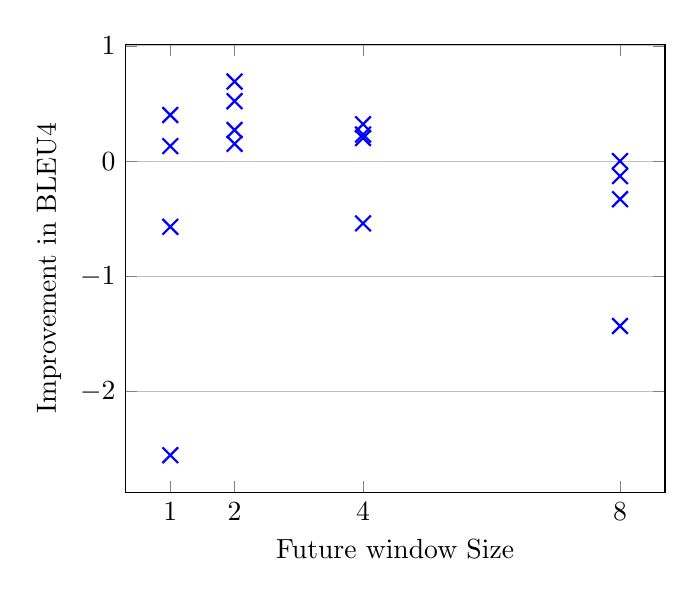
\begin{tikzpicture}
\begin{axis}[
    xlabel={Future window Size},
    ylabel={Improvement in BLEU4},
    xtick={0,1,2,4,8},
    ymajorgrids=true,
    % grid style=dashed,
]

\addplot[
    color=blue,
    mark=x,
    only marks,
    thick,
    mark size=4pt
    ]
    coordinates {
    (1, 0.4)(1, 0.13)(1,-0.57)(1,-2.55)(2,0.27)(2,0.52)(2,0.15)(2,0.69)(4,0.2)(4,0.23)(4,0.32)(4,-0.54)(8,0)(8,-0.13)(8,-1.43)(8,-0.33)
    };
    
\end{axis}
\end{tikzpicture}
\caption{Magnitude of improvement in BLEU4 scores between models trained from a pretrained model over training from scratch. We group models based on their future n-gram prediction window sizes. For example, for a model trained on past-future n-gram prediction of window size 2 for both past and future, the model trained from a pretrained model had an improvement of 0.52 over the model trained from scratch}
\label{fig:difference_bleu_pretrained_from_scratch}
\end{figure}

\subsection{Effectiveness of using sequence level knowledge distillation}
As collaborated in many other work in non-autoregressive literature \cite{ren_study_2020_comma, gu_non-autoregressive_2018, gu_levenshtein_2019, guo_non-autoregressive_2020_image_captioning, bao_non-autoregressive_2019_position_learning, wang_semi-autoregressive_2018,saharia_non-autoregressive_2020_latent_alignment, chan_kermit_2019, chan_multilingual_kermit, ghazvininejad_mask-predict_2019,stern_insertion_2019, zhou_improving_2020_with_monolingual_data, ran_guiding_2020_reordering, ma_flowseq_2019, qian_glancing_2020, guo_fine-tuning_2019_curriculum, ding_context-aware_2020}, models trained on distilled data for non-autoregressive machine translation performed significantly better than original data. From our experiments, the difference in BLEU4 score between the model trained on distilled data and its model counterpart trained on original data assumes an almost linear relationship. This relationship is shown in Figure \ref{fig:difference_bleu_distill_original}. 

%plot difference in bleu4 score
\begin{figure}
\centering
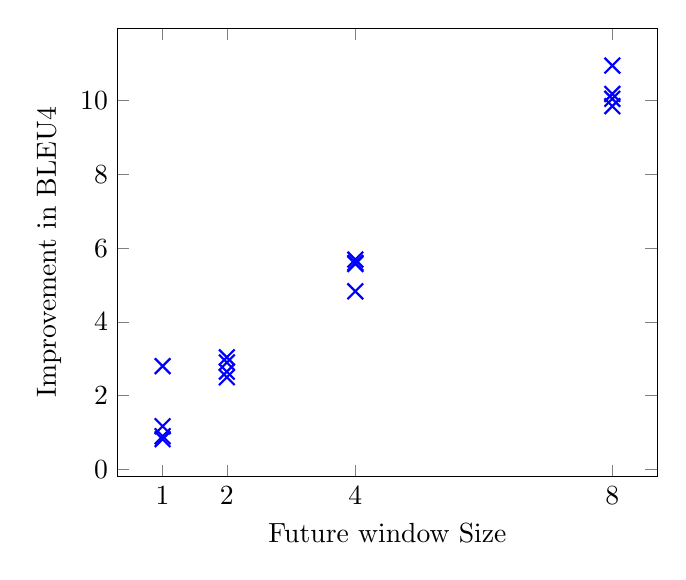
\begin{tikzpicture}
\begin{axis}[
    xlabel={Future window Size},
    ylabel={Improvement in BLEU4},
    xtick={0,1,2,4,8},
    % ymajorgrids=true,
    % grid style=dashed,
]

\addplot[
    color=blue,
    mark=x,
    only marks,
    thick,
    mark size=4pt
    ]
    coordinates {
    (1, 0.9)(1,1.17)(1,0.82)(1,2.8)(2,2.9)(2,2.65)(2,2.5)(2,3.04)(4,5.6)(4,5.57)(4,4.83)(4,5.69)(8,10.95)(8,9.85)(8,10.18)(8,10.05)
    };
    
\end{axis}
\end{tikzpicture}
\caption{Magnitude of improvement in BLEU4 scores between models trained on distilled over original data. We group models based on their future n-gram prediction window sizes. For example, for a model trained on past-future n-gram prediction of window size 4 for both past and future, the model trained on distilled data achieved an improvement of 5.6 in BLEU score.}
\label{fig:difference_bleu_distill_original}
\end{figure}



\section{Effect of Decoding Methods} 
As noted in Section \ref{sec:decoding_methods}, we use several methods for decoding during inference. These methods include argmax decoding, beam search of beam length 1 to 4, and hysteresis decoding.

\subsection{Argmax Decoding}
Argmax Decoding is the most straightforward decoding method. In our experiments, unless stated, argmax decoding is the default method. At each decoding step, the most probable token(s) is chosen as the generated token. Our results using argmax decoding are shown in Table \ref{tab:4.5_distill_vs_original_results}. Argmax decoding works well for the prediction of the future window. However, as noted in Section \ref{subsec:effective_argmax}, argmax decoding is too naive for sequence refinement. Therefore, we introduce hysteresis decoding for sequence refinement.

\subsection{Beam Search}
Beam search also consistently improves the BLEU score across all settings. Beam search can also be used in complement with both argmax decoding and hysteresis decoding. Take note that beam size of 1 is equivalent to simple argmax decoding. We show the results for models trained on distilled data, without any sequence refinement, at Table \ref{tab:beam_search_results_npe}. 

\begin{table}[]
\centering
\begin{tabular}{|c|c|c|cccc|}
\hline
\begin{tabular}[c]{@{}c@{}}Future \\ Window Size\end{tabular} & setting      & training task & beam1 & beam2 & beam3 & beam4  \\ \hline
8                                                             & from scratch & past-future   & 18.89 & 19.03 & 19.09 & 19.09  \\ \cline{3-7} 
8                                                             & from scratch & future-only   & 19.63 & 19.73 & 19.77 & 19.78  \\ \cline{2-7} 
8                                                             & pretrained   & past-future   & 17.66 & 18.08 & 18.17 & 18.19  \\ \cline{3-7} 
8                                                             & pretrained   & future-only   & 19.50  & 19.67 & 19.72 & 19.73  \\ \hline
4                                                             & from scratch & past-future   & 22.65 & 23.05 & 23.12 & 23.19  \\ \cline{3-7} 
4                                                             & from scratch & future-only   & 23.55 & 23.73 & 23.79 & 23.82  \\ \cline{2-7} 
4                                                             & pretrained   & past-future   & 22.88 & 23.18 & 23.28 & 23.3   \\ \cline{3-7} 
4                                                             & pretrained   & future-only   & 23.87 & 23.82 & 23.87 & 23.9   \\ \hline
2                                                             & from scratch & past-future   & 25.50  & 25.73 & 25.84 & 25.84  \\ \cline{3-7} 
2                                                             & from scratch & future-only   & 25.76 & 25.8  & 25.85 & 25.883 \\ \cline{2-7} 
2                                                             & pretrained   & past-future   & 25.78 & 26.01 & 26.11 & 26.13  \\ \cline{3-7} 
2                                                             & pretrained   & future-only   & 26.45 & 26.57 & 26.6  & 26.59  \\ \hline
1                                                             & from scratch & past-future   & 27.01 & 27.11 & 27.27 & 27.35  \\ \cline{3-7} 
1                                                             & from scratch & future-only   & 26.94 & 27.29 & 27.41 & 27.37  \\ \cline{2-7} 
1                                                             & pretrained   & past-future   & 27.44 & 27.61 & 27.6  & 27.54  \\ \cline{3-7} 
1                                                             & pretrained   & future-only   & 26.37 & 26.47 & 26.49 & 26.49  \\ \hline
\end{tabular}
\caption{BLEU4 scores of models decoded using argmax decoding and beam search of size 1, 2, 3 and 4, and without doing sequence refinement. Future window size refers to the window size of the future n-gram prediction. Setting refers to the model being trained from scratch, or from a pretrained model using transfer learning. Training task refers to the task the model is trained on, which is either the past-future n-gram prediction task, or the future-only n-gram prediction task.}
\label{tab:beam_search_results_npe}
\end{table}

\begin{figure}[hpbt!]
    \centering
    \includegraphics{images/chap04_images/beam_search_improvements.pdf}
    \caption{Improvement of BLEU4 score over beam size 1 when using a higher beam length 2, 3, 4. The darker the shade of green, the higher the improvement. For example, the model in the first row has an improvement of 0.14 in BLEU4 when decoding with beam search 2.}
    \label{fig:beam_search_improvement}
\end{figure}

From our experiments, beam search of increasing beam sizes performs consistently better than when using beam size of 1. These improvements in performance is depicted using color coding in Figure \ref{fig:beam_search_improvement}.

\subsection{Hysteresis Decoding} 
As previously introduced in Section \ref{subsec:hysteresis_decoding}, Hysteresis decoding is a decoding method aimed to improve sequence refinement using the past prediction window of the n-gram prediction task. There are two settings for which we can perform hysteresis decoding, by using a range, or by tweaking the low and high thresholds of the hysteresis decoding.


\subsubsection{Range Hysteresis Decoding} \label{subsubsec:range_hdec}

\begin{figure}[hpbt!]
    \centering
    \includegraphics[width=\textwidth]{images/chap04_images/hysteresis_decoding_range.pdf}
    \caption{BLEU4 score of models decoded using the range setting. For example, a model trained from scratch on 8/8 past and future n-gram prediction task on distilled data scored a BLEU4 score of 18.25, an improvement over its argmax decoding BLEU4 score of 18.13.}
    \label{fig:hysteresis_decoding_range}
\end{figure}

We use a range from 0.1 to 0.9 in intervals of 0.1. For example, if the hysteresis range is 0.2, and the probability of the candidate token is 0.50, the low and high threshold will be 0.30 and 0.70 respectively. We cap the highest and lowest probabilities to be compared against the candidate probability to be 0.95 and 0.05 respectively. This is to prevent the probabilities from going over 1.00 or under 0.


Our results are shown in Figure \ref{fig:hysteresis_decoding_range}. There is a clear benefit of BLEU score when using hysteresis decoding for large window sizes of 16. However, benefit seems to be reduced for smaller window sizes. Furthermore, the performance of the hysteresis decoding method seems to be independent from how wide the probability range is. Aside from a model trained on small window sizes (2/2), all models in our experiments yielded positive improvements when using range hysteresis decoding for sequence refinement.

\subsubsection{Manually setting high-low thresholds for Hysteresis Decoding} \label{subsubsec:manual_hdec}

\begin{figure}[hpbt!]

    \centering
    \includegraphics[width=\textwidth]{images/chap04_images/hysteresis_decoding_manual_2.pdf}
    \caption{Color coded lower triangular grid containing the BLEU4 score when decoding using a variety of low and high hysteresis thresholds for models trained from scratch. The darker the green/red, the better/worse the change in BLEU score. For example, for a window size of 8 each for past and future n-gram prediction window, trained on distilled data and from scratch, scored a BLEU4 score of 18.48 on a low threshold of 10 and a high threshold of 20 using hysteresis decoding. Without hysteresis decoding, the BLEU4 score is 18.13}
    \label{fig:hysteresis_decoding_manual_2}
\end{figure}
\begin{figure}[hpbt!]

    \centering
    \includegraphics[width=\textwidth]{images/chap04_images/hysteresis_decoding_manual_1.pdf}
    \caption{Color coded lower triangular grid containing the BLEU4 score when decoding using a variety of low and high hysteresis thresholds for models trained from a pretrained model. The darker the green/red, the better/worse the change in BLEU score. For example, for a window size of 8 each for past and future n-gram prediction window, trained on distilled data and from scratch, scored a BLEU4 score of 17 on a low threshold of 10 and a high threshold of 20 using hysteresis decoding. Without hysteresis decoding, the BLEU4 score is 16.70}
    \label{fig:hysteresis_decoding_manual_1}
\end{figure}


We run a lower triangular grid search of low probabilities of 0.1 to 0.8, and high probabilities of 0.2 to 0.9, all in intervals of 0.1. Our results are shown and color coded in both Figure \ref{fig:hysteresis_decoding_manual_2} and Figure \ref{fig:hysteresis_decoding_manual_1}. Note that when using manual settings for hysteresis decoding, the probability of the candidate token is largely ignored, and the probability histories are used as basis for replacement.

Similar to the observations in Section \ref{subsubsec:range_hdec}, we deduce that the benefits of hysteresis decoding are more pronounced as the window sizes get larger, and its benefits are diminished for smaller window sizes. At window size of 8/8, there is a clear increase of the improvement in BLEU score compared to window 2/2, and 4/4. There is also a noticeable improvement in BLEU score as the difference between low and high threshold increases. This suggests the decoding process benefits from using surrounding tokens as a scaffolding to gauge the legitimacy of the generated token.

\subsection{Influence of freezing certain layers for transfer learning}
In order to understand the importance of the information in each layer to non-autoregressive sequence generation, we tried freezing different layers during transfer learning to determine the impact of training these layers. We conduct our experiments using a window size of 1/1 for the past-future ngram prediction task.

\subsubsection{Effect of freezing the encoder}

\begin{table}[]
\begin{tabular}{c|c|c|c|c|c|c|}
\cline{2-7}
                                     & \multicolumn{6}{c|}{Trainable Decoder Layer(s)}                          \\ \cline{2-7} 
                                     & 0, 1, 2, 3, 4, 5 & 1, 2, 3, 4, 5 & 2, 3, 4, 5 & 3, 4, 5 & 5, 4   & 5     \\ \hline
\multicolumn{1}{|c|}{frozen encoder} & 7.29             & 6.99          & 6.71       & 6.01    & 4.97   & 3.51  \\
\multicolumn{1}{|c|}{\% change}      & -73.43           & -74.52        & -75.54     & -78.09  & -81.88 & -87.2 \\ \hline
\end{tabular}
\caption{BLEU4 and percentage decrease in BLEU4 score when freezing the encoder and updating the decoder. These models use a window size of 1/1.}
\label{tab:freeze_encoder_results}
\end{table}

We freeze the encoder by not allowing any updates on the weights of the encoder during training. The decoder is still trained and updated as normal. 

Our results are shown at Table \ref{tab:freeze_encoder_results}. We find that freezing the encoder resulted in a catastrophic drop in performance. Therefore, we focus on freezing different layers in both the decoder and the encoder.


% \subsubsection{Effect of freezing the decoder}
% We train the encoder and freeze the decoder by not allowing the weights of the decoder to be updated during training. We find that freezing the 

\subsubsection{Importance of the position of trained layers for transfer learning}

\begin{table}[]
\centering
\begin{tabular}{c|c|c|c|}
\cline{2-4}
\multicolumn{1}{l|}{}            & \multicolumn{3}{c|}{Layers trained} \\ \cline{2-4} 
                                 & d05e05   & d0145e0145  & d5e012345  \\ \hline
\multicolumn{1}{|c|}{window 1/1} & 18.76    & 23.37       & 23.21      \\
\multicolumn{1}{|c|}{\% decline} & -31.63   & -14.83      & -15.42     \\ \hline
\multicolumn{1}{|c|}{window 2/2} & 14.79    & 19.66       & 19.9       \\
\multicolumn{1}{|c|}{\% decline} & -42.56   & -23.65      & -22.72     \\ \hline
\multicolumn{1}{|c|}{window 4/4} & 7.62     & 13.62       & 17.11      \\
\multicolumn{1}{|c|}{\% decline} & -66.46   & -40.05      & -24.69     \\ \hline
\end{tabular}
\caption{Decline in BLEU4 score when freezing certain layers. For example, d5e012345 means that the 5th layer of the decoder and the layers 0-5 of the encoder are trained, and the rest of the layers (layer 0-4 of the decoder) are frozen.}
\label{tab:freeze_layers_results}
\end{table}


For adapting autoregressive models to non-autoregressive models, we find that choosing the right layers to train is more important than the actual number of layers train. For instance, we find that the encoders' layers are the most important layers to be trained. we can freeze most of the decoder layers and minimize the impact on the BLEU4 score. We also find the layers closer to the input and output are the most important layers to be trained. Our results are shown in Table \ref{freeze_layers_results}

\textcite{ethayarajh-2019-contextual_ani} showed in their experiments that contextualized representations are anisotrophic in all inputs layers and higher layers. That means that the representations occupy a narrow cone in the vector space. We hypothesize that the anisotrophic property is not beneficial for non-autoregressive sequence generation. We leave the testing of this hypothesis up to future work.

\chapter{Conclusions and Future Work}
\section{Concluding Remarks}

In this work, we have examined the potential of using transfer learning for non-autoregressive sequence generation in machine translation. We introduce a straightforward architecture involving adapter modules to adapt current autoregressive models to new non-autoregressive models via transfer learning. Next, we propose a novel decoding method, the hysteresis decoding method, to aid in sequence refinement and help improve BLEU scores at higher window sizes. Finally, we examine the contribution of different layers to non-autoregressive sequence generation.

This work has provided some insight into the workings of non-autoregressive sequence models, and how its limitations can possibly be tackled in future work.


\subsection{Future Work}
As seen in our experiments, the layers that seem to be the most instrumental to non-autoregressive decoding are the first few and last few layers of the transformer encoder. Therefore, it might be a good idea to supplement the encoder with external knowledge. One potential area of research is to incorporate graph embeddings into the encoder. 

\subsubsection{Application to other tasks}
Other than machine translation, other unexplored applications for non-autoregressive sequence generation tasks include automated audio captioning. Automated audio captioning applications often require real time captioning, hence there is a need for speed. However, it is slightly different from the work in this task, and the input would be preprocessed log-mel spectrograms, instead of word piece embedddings like in text. 

    
% Include appendix      % Set this up if needed
%\appendix

% Insert bibliography here
\printbibliography

\end{document}

% End of document
%-----------------------------------------------------------------------------------------------------